\documentclass[xcolor=pdftex,dvipsnames]{beamer}

\usepackage{amsmath}
\usepackage{amssymb}

\usepackage{comment}
\usepackage{textcomp}

\title{Microeconomic Theory --- ECON 323 503 \\ Chapter 8: Competitive 
  firms and markets}
\author{Vikram Manjunath}       %
\institute{Texas A\&M University}
\setbeamertemplate{navigation symbols}{}
\setbeamertemplate{footline}{}
\usefonttheme{serif}
\begin{document}

\maketitle

\begin{frame}
\frametitle{Outline}
\begin{enumerate}[<+->]
\item Perfect competition: firms cannot affect the price of a good on
  their own.
\item Profit maximization: how much to produce if at all.
\item Competition in the short run: supply curve is driven by variable
  costs.
\item Competition in the long run: no fixed costs and firms can
  enter/exit.
\end{enumerate}
\end{frame}




\begin{frame}
\frametitle{Perfect competitions}
\emph{Perfectly competitive} industry: firms are ``price takers.''
\bigskip

\uncover<2->{Price taking: cannot affect the price significantly.}
\bigskip


\uncover<3->{If there are many competing firms, raising your price causes demand
for your goods to drop to zero.}

\end{frame}





\begin{frame}
\frametitle{Perfect competition}
For firms to be price takers:
\begin{enumerate}[<+->]
\item There are many small firms.
\item These firms sell identical products.
\item Buyers are aware of the price charged by each of the firms.
\item There are no transaction costs: buyers can easily switch from one firm
  to another.
\item Firms can freely enter and exit the market.
\end{enumerate}
\uncover<6->{Example:  Chicago commodity exchange}
\end{frame}





\begin{frame}
\frametitle{Each firm faces a demand curve}
\emph{Residual demand:} For a given price, how much does the market
demand beyond what the \emph{other} firms are supplying?
\uncover<2->{\[
D^r(p) = D(p) - S^O(p)
\]}
\uncover<3->{$D(p)$ --- Market demand}
\bigskip

\uncover<4->{$S^O(p)$ --- \emph{Other} firms' supply (add up the supply of other firms).}



\end{frame}




\begin{frame}
\frametitle{Residual demand curve}
\begin{center}
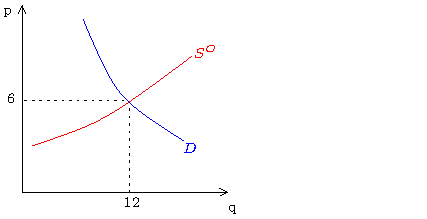
\includegraphics{pics/ResD1}
\end{center}

\end{frame}
\begin{frame}
\frametitle{Residual demand curve}
\begin{center}
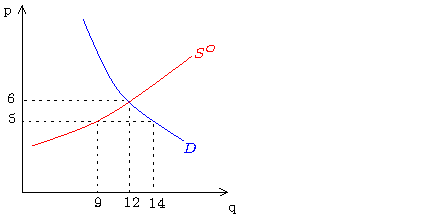
\includegraphics{pics/ResD2}
\end{center}

\end{frame}


\begin{frame}
\frametitle{Residual demand curve}
\begin{center}
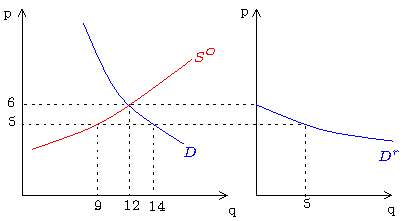
\includegraphics{pics/ResD3}
\end{center}

\end{frame}





\begin{frame}
\frametitle{Residual demand curve}
The demand curve that a single firm faces is a lot flatter than the
market demand.

\bigskip

\uncover<2->{ In fact, it is a lot less elastic: Let $\varepsilon_i$ be the
 elasticity of firm $i$'s (residual) demand curve.
\[
\varepsilon_i = n\varepsilon - (n-1)\eta_O
\]}
\bigskip

\uncover<3->{$n$ --- number of identical firms.}
\bigskip

\uncover<4->{$\varepsilon$ --- demand elasticity.}
\bigskip

\uncover<5->{$\eta_O$ --- other firms' supply elasticity.}
\bigskip

\uncover<6->{(Differentiate $D^r(p) = D(p) - S^O(p)$ with respect to $p$.)}

\end{frame}

\begin{frame}\frametitle{An example}
Number of firms, $n=78$
\medskip

\uncover<2->{Market demand elasticity, $\varepsilon = -1.1$ (not too elastic)}
\medskip

\uncover<3->{Other firms' supply elasticity, $\eta_O = 3.1$}
\medskip

\uncover<4->{\[
\varepsilon_i = n\varepsilon - (n-1)\eta_O = 78\times (-1.1) - 77\times
3.1 = -324.5.
\]}

\uncover<5->{Residual demand for firm $i$ is over 300 times more elastic than
market demand!}


\end{frame}
\begin{frame}
\frametitle{The demand curve that a perfectly competitive firm faces}
\[\varepsilon_i = n\varepsilon - (n-1)\eta_O
\]
What happens as $n$ gets bigger and bigger?

\uncover<2->{\bigskip
$\varepsilon < 0$ and $\eta_O>0$. So, as $n$ grows,
$|\varepsilon_{i}|$ gets bigger.}

\bigskip
\uncover<3->{If there are an ``infinite'' number of competing firms, the demand curve
that a firm faces is \emph{perfectly elastic}: it's a horizontal line
at some price $p$.}

\bigskip
\uncover<4->{This means that the firm can sell as many units as it wishes to as
long as it charges no more than $p$. If it charges anything more than
$p$, demand for its good drops to zero.}
\bigskip

\uncover<5->{This is intuitive: if other firms sell the same product as you, when
you charge more than they do, nobody buys from you.}



\end{frame}


\begin{frame}
\frametitle{Importance of perfect competition}
\begin{enumerate}[<+->]
\item Many real world markets are \emph{close enough to} perfectly
  competitive that the predictions of the competitive model are
  reasonably accurate.
\item More importantly: the competitive model is a \emph{benchmark} to
  compare real world markets to. 
\end{enumerate}
\end{frame}





\begin{frame}
\frametitle{Profit maximization}
Profit at output $q$:
\[
\pi(q) = R(q)-C(q)
\]
\uncover<2->{$R$ --- revenue.}
\bigskip

\uncover<3->{$C$ --- cost.}
\bigskip

\uncover<4->{Since $C$ is \emph{economic} cost (including all opportunity costs),
$\pi$ is the \emph{economic} profit.}
\end{frame}





\begin{frame}
\frametitle{Two steps to maximizing profit}
When picking $q$:
\begin{enumerate}[<+->]
\item Which level $q^*$ yields the highest profit (or minimizes loss
  when $(\pi(q)<0)$?
\item Should you just shut down rather than produce $q^*$?
\end{enumerate}
\end{frame}

\begin{frame}\frametitle{Picking $q^*$}
\begin{center}
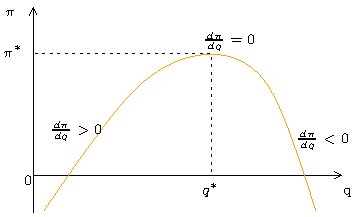
\includegraphics[scale=1.25]{pics/ProfMax}
\end{center}
\end{frame}



\begin{frame}
\frametitle{Output rules}
Three rules for picking $q^*$:
\begin{enumerate}[<+->]
\item Pick $q^*$ where $\pi$ is maximized

\item Pick $q^*$ so \emph{marginal profit},$\frac{d\pi}{dq}$, is
  zero.
\item Pick $q^*$ so \emph{marginal revenue}, $\frac{d R}{dq}$,
equals \emph{marginal cost}, $\frac{d C}{dq}$.
\end{enumerate}
\uncover<4->{These are all equivalent.}
\end{frame}





\begin{frame}
\frametitle{Output rules}
Suppose that $q^*$ maximizes $\pi$.
\bigskip

\uncover<2->{Decreasing $q$ reduces profit: to the left of $q^*$,
$\frac{d\pi}{dq} > 0$.}
\bigskip

\uncover<3->{Increasing $q$ reduces profit: to the right of $q^*$,
$\frac{d\pi}{dq} < 0$.}

\bigskip
\uncover<4->{So, \emph{at} $q^*$, $\frac{d\pi}{dq} = 0$.}


\bigskip
\uncover<5->{$\frac{d\pi}{dq}$ is \emph{marginal profit}: the additional profit per
unit increase of quantity.}



\end{frame}





\begin{frame}
\frametitle{Output rules}
Since $\pi(q) = R(q) - C(q)$,
\[
\frac{d\pi(q)}{dq} = \frac{d R(q)}{dq}- \frac{d C(q)}{dq} = MR(q) - MC(q).
\]
\uncover<2->{$MR(q)$ is \emph{marginal revenue} at $q$: the additional revenue per
unit increase of quantity.}
\bigskip

\uncover<3->{$MC(q)$ is \emph{marginal revenue} at $q$: the additional cost per
unit increase of quantity.}
\bigskip

\uncover<4->{If $\frac{d\pi(q^*)}{dq} = 0$ then 
\[
MR(q^*) = MC(q^*).
\]}

\end{frame}





\begin{frame}
\frametitle{Second order condition}
Remember that ``$\frac{d\pi(q^*)}{dq}= 0$'' is the \emph{first order
  condition}.

\bigskip

\uncover<2->{This guarantees that $q^*$ maximizes profit only when the profit
function is ``concave'' so that $\frac{d^2\pi(q)}{dq^2}< 0$.}
\bigskip

\uncover<3->{This is the \emph{second order condition}.}
\bigskip

\uncover<4->{It is equivalent to $\frac{dMR(q)}{dq} < \frac{dMC(q)}{dq}$: the
marginal revenue curve is flatter than the marginal cost curve }
\end{frame}





\begin{frame}
\frametitle{Shutdown rules}
What happens if $\pi(q^*) < 0$ so that you're running a loss?

\bigskip

\uncover<2->{Should you shut down?}

\bigskip

\uncover<3->{Only if doing so reduces your loss.}

\end{frame}





\begin{frame}
\frametitle{Example}
$R= \$2,000$

$C = VC + F$

$VC = \$1,000$

$F = \$3,000$.
\bigskip

\uncover<2->{
Then 
\[
\pi = R- C = R-VC-F = \$2,000 - \$1,000- \$3,000 = -\$2,000.
\]}

\uncover<3->{You're running a loss of $\$2,000$. Should you shut down?}
\bigskip

\uncover<4->{No.}
\bigskip

\uncover<5->{If you shut down, $R=\$0$ and $VC=\$0$ so $\pi = -\$3,000.$}
\end{frame}





\begin{frame}
\frametitle{Competition in the short run}
Demand curve that the firm faces is horizontal. 
\bigskip

\uncover<2->{How much does revenue rise if you sell on more unit? }
\bigskip

\uncover<3->{By $p$,the price.}
\bigskip

\uncover<4->{So $MR(q) = p$ for every $q$.}
\end{frame}





\begin{frame}
\frametitle{Finding $q^*$}
To find $q^*$, equate MR and MC to find optimal quantity:

\[
MR(q^*) = MC(q^*)
\]
\uncover<2->{So \[MC(q^*) = p.\]}

\uncover<3->{The second order condition tells us that 
\[
\frac{dMC}{dq}>0
\]}
\uncover<4->{So, $MC$ is upward sloping.}

\end{frame}


\begin{frame}
\frametitle{Finding $q^*$}
\begin{center}
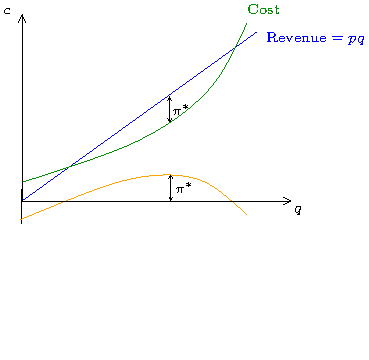
\includegraphics{pics/CRProf1}
\end{center}

\end{frame}
\begin{frame}
\frametitle{Finding $q^*$}
\begin{center}
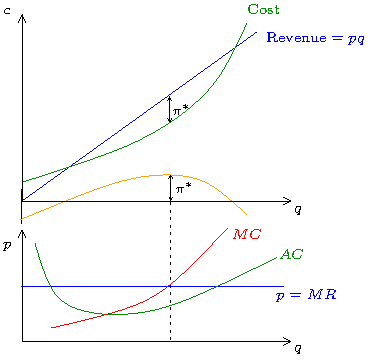
\includegraphics{pics/CRProf2}
\end{center}
\end{frame}



\begin{frame}
\frametitle{Finding $q^*$}
\begin{center}
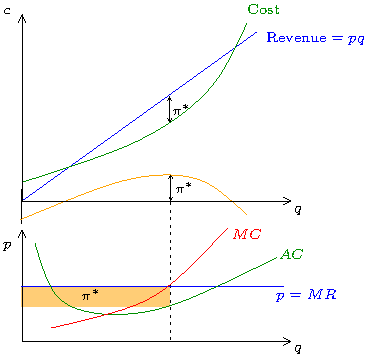
\includegraphics{pics/CRProf}
\end{center}

\end{frame}





\begin{frame}\frametitle{Shut down or not?}
Three cases:
\begin{enumerate}[<+->]
\item $\text{minimum AC}< p$: you're making money stay in business.
\item $\text{minimum AVC} \leq p \leq \text{minimum AC}$: you're running a
  loss, but reducing it by staying in business.
\item $p > \text{minimum AVC}$: you're losing money by staying in
  business. Shut down.
\end{enumerate}
\end{frame} 





\begin{frame}\frametitle{Short run supply}
Remember, for $p\geq\text{minimum AVC}$,
\[
p=MC(q^*).
\] and for $p<\text{minimum AVC}$, output is zero.

\bigskip

\uncover<2->{That's your supply curve!}
\end{frame} 

\begin{frame}\frametitle{Short run supply curve}
\begin{center}
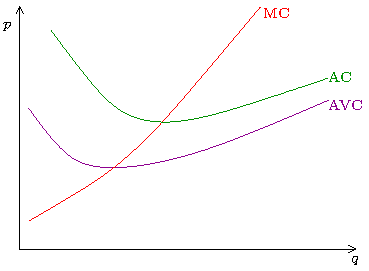
\includegraphics{pics/Supply1}
\end{center}

\end{frame}

\begin{frame}\frametitle{Short run supply curve}
\begin{center}
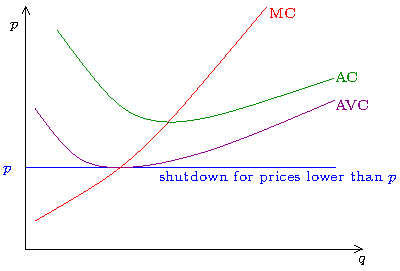
\includegraphics{pics/Supply2}
\end{center}

\end{frame}

\begin{frame}\frametitle{Short run supply curve}
\begin{center}
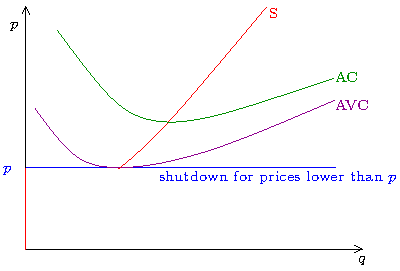
\includegraphics{pics/Supply3}
\end{center}

\end{frame}



\begin{frame}\frametitle{Changes in factor prices}

What happens if the price of an input changes?
\bigskip

\uncover<2->{This increases VC.}
\bigskip

\uncover<3->{So AVC and MC curves are higher. Thus, the supply curve shifts
upwards.}
\uncover<4->{\begin{center}
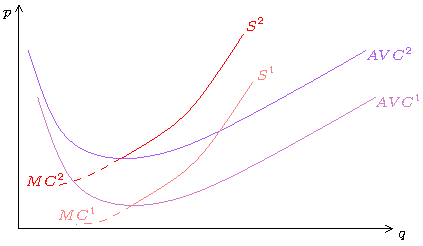
\includegraphics{pics/SupplyShift}
\end{center}}
\end{frame} 





\begin{frame}\frametitle{Short run market supply}
\begin{center}
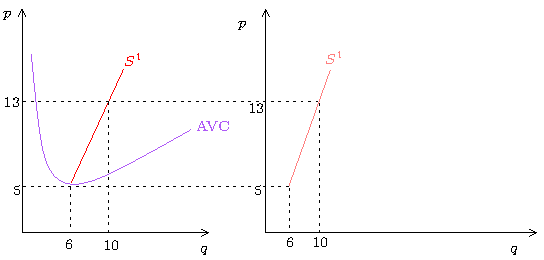
\includegraphics{pics/MarketSupply1}
\end{center}
If there's only one firm, its supply is the market supply.
\end{frame} 

\begin{frame}\frametitle{Short run market supply}
\begin{center}
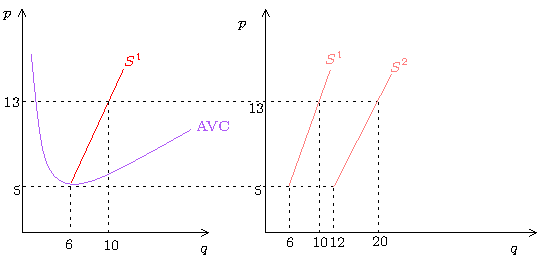
\includegraphics{pics/MarketSupply2}
\end{center}
If there are two, add them up.
\end{frame} 

\begin{frame}\frametitle{Short run market supply}
\begin{center}
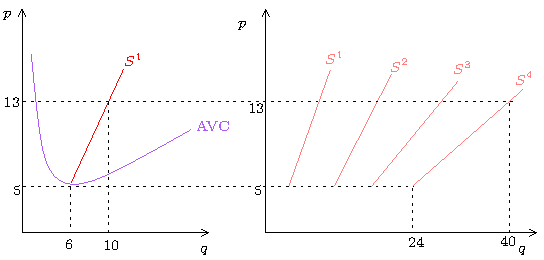
\includegraphics{pics/MarketSupply3}
\end{center}
And so on.
\end{frame} 





\begin{frame}\frametitle{What if the firms aren't identical}
\begin{center}
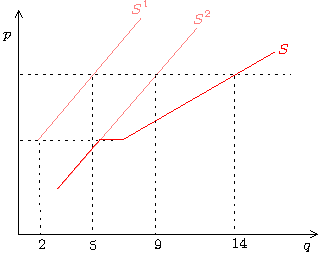
\includegraphics{pics/AsymMarketSupply}
\end{center}
 You can still add supply curves horizontally.
\end{frame} 





\begin{frame}\frametitle{Short run competitive equilibrium}
\begin{center}
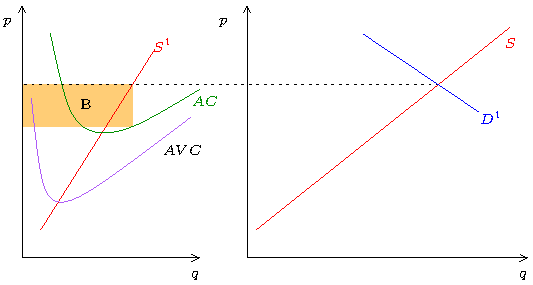
\includegraphics{pics/Equilibrium1}
\end{center}
Firms are making a profit (B).
\end{frame} 





\begin{frame}\frametitle{Short run competitive equilibrium}
\begin{center}
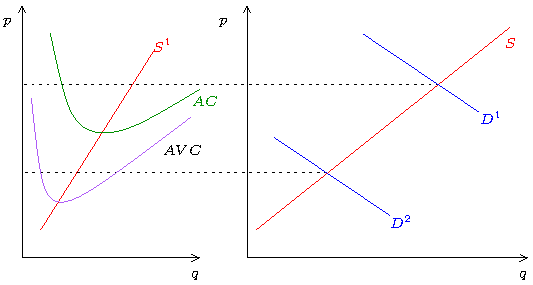
\includegraphics{pics/Equilibrium2}
\end{center}
Equilibrium price shifts if demand changes.
\end{frame} 


\begin{frame}\frametitle{Short run competitive equilibrium}
\begin{center}
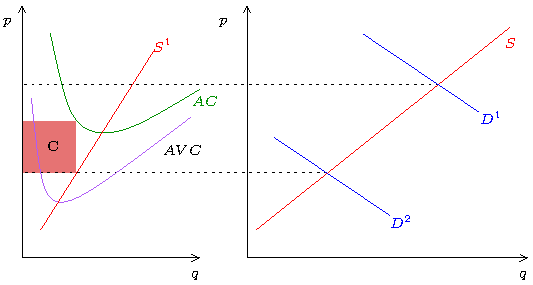
\includegraphics{pics/Equilibrium3}
 \end{center}
Firms are making a loss (C) but covering variable costs.
\end{frame} 




\begin{frame}\frametitle{Competition in the long run}
Everything can be varied in the long run.

\bigskip
\uncover<2->{Shut down in case of loss.}
\end{frame} 


\begin{frame}\frametitle{Competition in the long run}
Long run: pick $q^*$ and  inputs to maximize profit based on
\emph{forecast} of future.

\uncover<2->{
\bigskip

What if forecast is wrong?}
\bigskip

\uncover<3->{ Stuck with wrong input in short run. It takes time to fix it.}
\bigskip

\uncover<4->{ Again, in the long run, the firm can have the right inputs.}
\end{frame}





\begin{frame}
\frametitle{An example}
\begin{center}
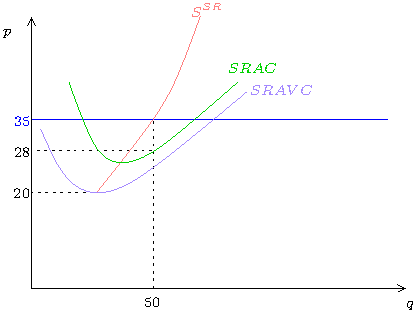
\includegraphics{pics/LRS1}
\end{center}
Stuck with small a plant: at $p=\$35,$ produce 50 units. \\

\
\end{frame}


\begin{frame}
\frametitle{An example}
\begin{center}
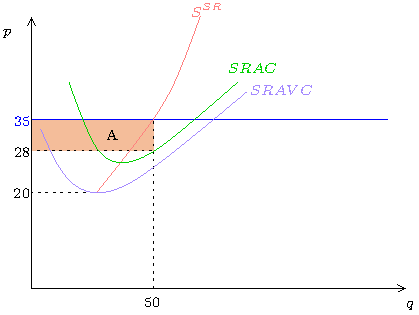
\includegraphics{pics/LRS2}
\end{center}
Stuck with small a plant: at $p=\$35,$ produce 50 units. 

Profit is A.
\end{frame}


\begin{frame}
\frametitle{An example}
\begin{center}
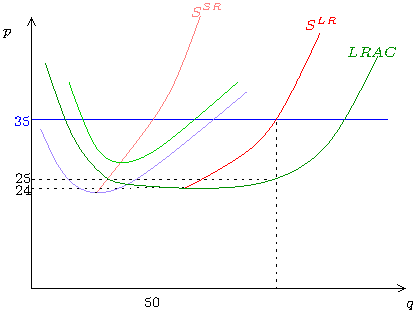
\includegraphics{pics/LRS3}
\end{center}
With optimal plant size: at $p=\$35,$ produce 100 units. \\

\
\end{frame}

\begin{frame}
\frametitle{An example}
\begin{center}
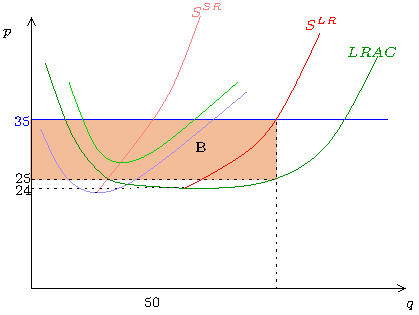
\includegraphics{pics/LRS4}
\end{center}
With optimal plant size: at $p=\$35,$ produce 100 units. 

Profit is B.
\end{frame}








\begin{frame}
\frametitle{Long-run market supply}
Just like short run: just add each firm's supply curve horizontally to
get market supply.
\bigskip

\uncover<2->{\emph{Important difference:} number of firms is fixed in short run.
\bigskip}

\uncover<3->{ Entry/exit is free in long run.}

\bigskip
\uncover<4->{
Another difference: prices of inputs respond to increased market output.}


\end{frame}








\begin{frame}
\frametitle{Role of entry/exit}
In the long run:
\begin{itemize}[<+->]
\item Enter if $\pi > 0$.
\item Exit  if $\pi < 0$.
\end{itemize}

\bigskip
\uncover<3->{
\emph{Major implication:} Long run profit is zero.}

\bigskip
\uncover<4->{ Remember: this is economic profit. The cost is \emph{all} economic
cost, including opportunity cost.}
\end{frame}








\begin{frame}
\frametitle{Role of entry}
The \emph{ marginal firm} makes no profit:
\bigskip

\uncover<2->{ If demand shifts right, profits of existing firms go up.}
\bigskip

\uncover<3->{ As entry is free, new firms enter: there's money to be made.}
\bigskip

\uncover<4->{ More firms means rightward shift of market supply.}
\bigskip

\uncover<5->{ Price falls and profit goes down.}

\bigskip
\uncover<6->{ As long as there's money to be made, firms keep popping up.}

\bigskip
\uncover<7->{ If the last firm that enters makes no profit, no more firms enter.}



\end{frame}








\begin{frame}
\frametitle{Role of exit}
The \emph{marginal firm} makes no loss:

\bigskip
\uncover<2->{ If demand shifts left, profits of existing firms drop, possibly so
much that they are now making losses.}

\bigskip

\uncover<3->{ As exit is free, firms under loss shut down.}
\bigskip

\uncover<4->{ Fewer firms means leftward shift of market supply.}
\bigskip


\uncover<5->{ Price rises and profits increase (losses decrease).}
\bigskip

\uncover<6->{ As long as they're losing money, firms keep dropping out.}
\bigskip

\uncover<7->{ Once there is no more loss, no more firms exit.}


\end{frame}








\begin{frame}
\frametitle{When entry is not free}
\begin{enumerate}[<+->]
\item Start-up costs: utilities.
\item Licensing: cabs.
\item Limited resources for inputs: wireless spectrum  for mobile phones.

\end{enumerate}
\end{frame}








\begin{frame}
\frametitle{Long-run market supply with free entry}
If an \emph{unlimited} number of firms have
\begin{enumerate}[<+->]
\item identical costs
\item free entry/exit
\item fixed input prices
\end{enumerate}

\uncover<4->{ then market supply is a horizontal line at minimum average cost.}
\end{frame}








\begin{frame}
\frametitle{Long-run market supply with free entry}
\begin{center}
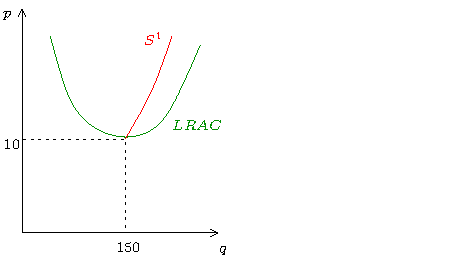
\includegraphics{pics/LRMS1}
\end{center}
$S^1$ is the supply curve of a single firm. Obviously market supply is
zero below \$10.
\end{frame}


\begin{frame}
\frametitle{Long-run market supply with free entry}
\begin{center}
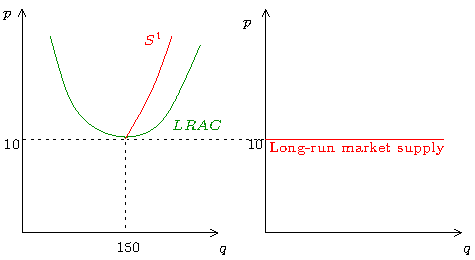
\includegraphics{pics/LRMS2}
\end{center}
If $p>\$10$ then  $\pi>0$. \uncover<2->{Firms enter until $p=\$10$.}\\
\uncover<3->{At $p=\$10$, $Q=n\times 150$ for any number of firms $n$.}
\end{frame}








\begin{frame}
\frametitle{If the three conditions aren't met}
\begin{enumerate}[<+->]
\item No free entry: Just like short run, market supply slopes
  upwards.
\item Firms differ: at low price, only low cost firms active. If these
  are limited in number, market supply slopes upwards. Otherwise, it's
  horizontal.
\item Input prices vary with market output: 

\begin{enumerate}\uncover<4->{\item price rises with
output: market supply slopes upwards. }
\uncover<5->{\item price drops
  with output:market supply slopes downwards.}
\end{enumerate}
\end{enumerate}
\end{frame}








\begin{frame}
\frametitle{Long-run market supply in an increasing-cost market}
\begin{center}
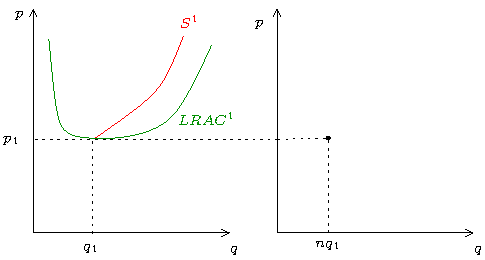
\includegraphics{pics/ICM1}
\end{center}
At price $p_1$, each firm produces $q_1$. If there are $n$ firms,
market supply is $Q_1=nq_1$.
\end{frame}

\begin{frame}
\frametitle{Long-run market supply in an increasing-cost market}
\begin{center}
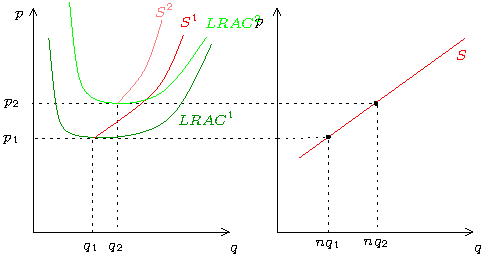
\includegraphics{pics/ICM2}
\end{center}
At $Q_2=nq_2 > Q_1$, the input is more expensive. So the cost curves
all shift up and  $S$ slopes upwards.
\end{frame}








\begin{frame}
\frametitle{Long-run supply curve with trade}
Many goods are traded on world markets: oil, minerals, machinery, etc.

\bigskip
\uncover<2->{$S(p)$ --- total world supply.}
\bigskip

\uncover<3->{$D^O(p)$ --- total demand outside of a country.
}
\bigskip

\uncover<4->{ Residual supply:
\[
S^r(p) = S(p) - D^O(p)
\]}
\uncover<5->{ From the perspective of consumers in that country, the supply of the
good is $S^r$}.

\end{frame}


\begin{frame}
\frametitle{Residual supply}
\begin{center}
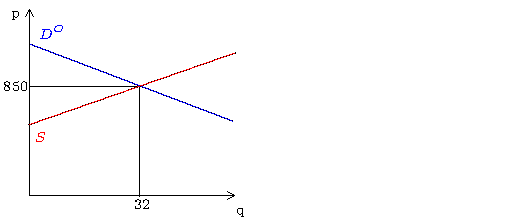
\includegraphics{pics/ResS1}
\end{center}

When $p=\$850$, the rest of the world consumes the entire world
supply. This leaves a supply of 0 for the country.
\end{frame}
\begin{frame}
\frametitle{Residual supply}
\begin{center}
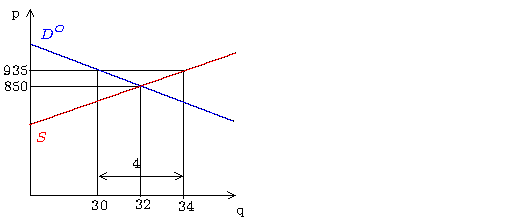
\includegraphics{pics/ResS2}
\end{center}

At $p=\$935$, the rest of the world demands 30 units
and the world supply is 30 units, leaving a supply of 4 for the country.
\end{frame}


\begin{frame}
\frametitle{Residual supply}
\begin{center}
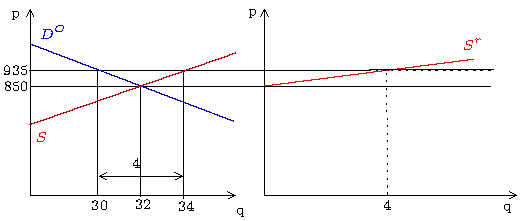
\includegraphics{pics/ResS3}
\end{center}

Doing this for all prices above \$850 gives us $S^r$.\\
It's a lot flatter than $S$.
\end{frame}



\begin{frame}
\frametitle{Elasticity of residual supply}
$\theta=\frac{Q_r}{Q}$ --- share of the total quantity consumed in the
country.\bigskip

\uncover<2->{$\eta$ --- market supply elasticity\bigskip}

\uncover<3->{$\varepsilon_O$ --- other countries' demand elasticity}


\uncover<4->{\[
\eta_r = \frac{\eta}{\theta} - \frac{1-\theta}{\theta} \varepsilon_O.
\]}

\uncover<5->{ Example: $\eta=0.5, \varepsilon=-0.7$ (estimates for world cotton
market).}
\medskip

\uncover<6->{ Low level of import: If $\theta=0.1\%$ then  $\eta_r=1,199.3$.}
\medskip

\uncover<7->{ Consumers in this country face a very flat supply curve.}
\medskip

\uncover<8->{ High level of import: If $\theta = 18.5\%$ then $\eta_r = 5.8$.}
\medskip

\uncover<9->{ Consumers in this country face an upward sloping supply curve.}

\end{frame}



\begin{frame}
\frametitle{Long-run competitive equilibrium}
Long run market supply is a horizontal line at the minimum average
cost.

\bigskip
\uncover<2->{Shifts in demand only change the quantity and not price.}

\bigskip

\uncover<3->{$S^{SR} \neq S^{LR}$ so equilibrium is different in short and long
run.}
\bigskip

\uncover<4->{$S^{SR}$ most likely slopes upwards.}
\end{frame}



\begin{frame}
\frametitle{Short-run and long-run competitive equilibrium}
\begin{center} 
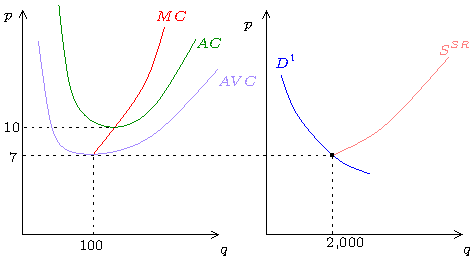
\includegraphics{pics/SRLREqu1}
\end{center}
Minimum $AVC = \$7$, 20 firms in short run, each with the right number
of level of fixed input for the long run.
\uncover<2->{When demand is  low, firms stay in
business but sell goods at a loss ($p=\$7$).}

\end{frame}

\begin{frame}
\frametitle{Short-run and long-run competitive equilibrium}
\begin{center}
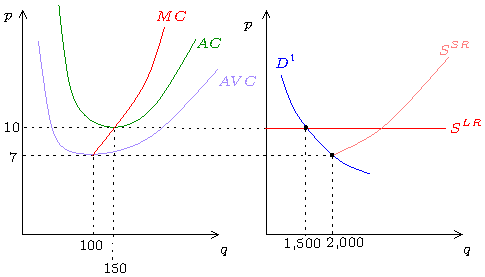
\includegraphics{pics/SRLREqu2} 
\end{center}
Minimum $AC=\$10$ so firms start going out of business in long run and
equilibrium quantity drops. \uncover<2->{So long-run price is higher than short-run price.}

\end{frame}


\begin{frame}
\frametitle{Short-run and long-run competitive equilibrium}
\begin{center}
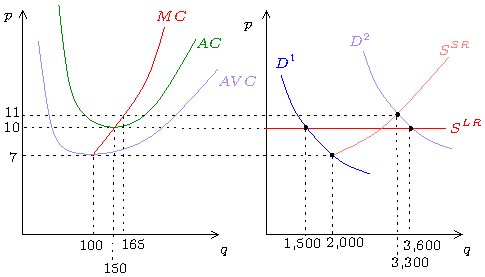
\includegraphics{pics/SRLREqu3}
\end{center}
Relationship is reversed
for high demand. Equilibrium price is higher in short run than in long
run.
\uncover<2->{Firms enter in the long run because short term price is high.}
\end{frame}


\end{document}






